\documentclass{article}


\usepackage{arxiv}

\usepackage[utf8]{inputenc} % allow utf-8 input
\usepackage[T1]{fontenc}    % use 8-bit T1 fonts
\usepackage{hyperref}       % hyperlinks
\usepackage{url}            % simple URL typesetting
\usepackage{booktabs}       % professional-quality tables
\usepackage{amsfonts}       % blackboard math symbols
\usepackage{nicefrac}       % compact symbols for 1/2, etc.
\usepackage{microtype}      % microtypography
\usepackage{lipsum}
\usepackage{graphicx}
\graphicspath{ {./images/} }


\title{Are we measuring what we think we are? Motivations and challenges of measuring the usage and impact of software designed for biomedical research}


\author{
 Ziyue Qi \\
  School of Coumputing and Information\\
  University of Pittsburgh\\
  Pittsburgh, PA 15213 \\
  \texttt{ziq2@pitt.edu} \\
  %% examples of more authors
   \And
 Zixuan Lu \\
  School of Coumputing and Information\\
  University of Pittsburgh\\
  Pittsburgh, PA 15213 \\
  \texttt{ZIL50@pitt.edu} \\
  \And
 Yuchen Lu \\
  School of Coumputing and Information\\
  University of Pittsburgh\\
  Pittsburgh, PA 15213 \\
  \texttt{yul217@pitt.edu} \\
  %% \AND
  %% Coauthor \\
  %% Affiliation \\
  %% Address \\
  %% \texttt{email} \\
  %% \And
  %% Coauthor \\
  %% Affiliation \\
  %% Address \\
  %% \texttt{email} \\
  %% \And
  %% Coauthor \\
  %% Affiliation \\
  %% Address \\
  %% \texttt{email} \\
}

\begin{document}
\maketitle
\begin{abstract}
Software has become vital in the advancement of biology and medicine. Analysis of usage and impact metrics of such software can be very beneficial to determining user and community contributor engagement. Such knowledge can be useful in justifying additional funding, encouraging additional use, and identifying unexpected usage. Furthermore, it can help define improvement areas and assist with managing project resources. However, there are several challenges associated with assessing usage and impact, many of which vary widely depending on the type of software being evaluated. These challenges involve issues of distorted, exaggerated, understated, or misleading metrics, as well as ethical and security concerns.  More attention to the nuances, challenges, and considerations involved in capturing impact across the diverse spectrum of biological software is needed. Although there are principles that can be generally applicable, there is not a single metric or approach to effectively evaluate a software tool’s impact, as this depends on aspects of the tool, how it is used, and how one wishes to evaluate engagement. We propose generalizable guidelines, as well as strategies for various types of software and resources. We also highlight outstanding issues in the field regarding how we measure or evaluate software impact. To gain an understanding of the issues hindering such evaluations, as well as to determine what appears to be helpful, we performed a survey of participants involved with scientific software projects for the Informatics Technology for Cancer Research (ITCR) program funded by the National Cancer Institute (NCI). We also performed investigations of software among this scientific community and others to determine how often infrastructure that supports such evaluations is implemented.  Our findings can help scientific software developers make the most out of the evaluations of their software so that they can more fully reap the benefits of such assessments
\end{abstract}


% keywords can be removed
%\keywords{First keyword \and Second keyword \and More}


\section{Introduction}
Analysis of biomedical software usage and impact metrics can be very beneficial to determine how software is being used and by whom. However, infrastructure necessary to support the capture of metrics is not always established and metrics are not always analyzed in the most useful way due to various challenges. Additionally, developers may not know what infrastructure, tools, and methods exist to support such assessments.We aim to provide guidance about such evaluations of software impact and engagement so that software developers can overcome barriers and challenges. We will also discuss ethical considerations and challenges that still require solutions. Providing developers with more guidance and knowledge of engagement assessment holds the potential for developers to improve the use and utility of their tools, improve their chances of funding for future development, and ultimately lead to the development of even more useful software to advance science and medicine \cite{wratten_reproducible_2021}. 


\section{Software Design Informs Successful Software Evaluation}
\label{sec:headings}
Consideration for the purpose of scientific software, can lead to much more successful evaluations of that software. Computational tools are designed to support well-defined tasks or goals often called use cases \cite{gamma_design_1995} for specific sets of users called personas\cite{cooper_inmates_2004}. Efforts to evaluate the utility and impact of tools should be guided by clear understanding of these use cases and personas, as tools might be assessed in terms of how well they support identified classes of users in meeting identified goals. Assessments of impact metrics should also be relevant to the interest of the audience that might use such evaluations. For example, detailed metrics on the usage of individual functions might be highly-informative to system developers aiming to meet users’ needs, but such metrics may be far too granular to be of interest to funding agencies and collaborators.  Effective assessments consider use cases, personas, and audience(s) to determine which information should be collected and how it should be presented. 

There is no sole individual scheme for collecting metrics that fits every research software tool. Research software takes a wide variety of forms with varying levels of complexity, project maturity, and authorial control. The meaning of an individual set of metrics may shift across different tool contexts. For example, in a web application providing access to a variety of interconnected tools, it may be feasible to collect user metrics on a per-account basis, to track each tool usage individually, and to collect information about the type of data users tend to work with. With this type of tool, users will rarely have access to older versions of the project. Thus developers can add version updates and collect metrics with clarity about how usage changed with updates. On the other hand, for tools that must be run (and possibly installed)  locally, like lightweight open-source scripts, users may be using older versions of the software that they previously downloaded.  Here, the metrics on a per-version basis provide a much better representation of usage, such as the number of unique downloads. 

Because user metrics are ultimately constructed from data, it can be tempting to simply collect an exhaustive amount of data, and then select metrics, or construct composite ones, from among this. However, this can add complexity, and being truly exhaustive with user behaviors is generally not possible. There is also the risk that metrics are selected or constructed in a biased manner which warps the meaning of the data. Therefore, it may be wisest to select a well-curated set of metrics ahead of time, with the intention of specific hypothesis testing based on ultimately the evaluation of how well the software supports it’s intended goal for it’s indeed use cases and personas, with the stakeholder audience in mind. Consideration of the motivation of the audience for such use cases and personas can further delineate what metrics to evaluate. Motivations for measuring usage can be categorized as either intrinsic or extrinsic, based on the intended audience and goals. Intrinsic motivations seek metric data to understand how best to meet the goals of the tool development effort. In contrast, extrinsic motivations seek to demonstrate the value and utility of the tool to stakeholders and other external communities. 
\subsection{Intrinsic Motivations}

Intrinsic motivations typically revolve around accruing information that will support either tool optimization or future activities. Tool optimization can involve improving workflows, performance, usage, or usability. Improving workflows can involve identifying unexpected usage patterns, inefficiencies in pre- and post-processing or inadequacies in documentation or examples. Improving performance often involves identifying mismatches between default parameters and common usage, or evolution in the error profiles or volume of data that influence error profiles or run-time characteristics. Improving usage generally involves quantifying who the user-base is, where other possible users might lie, what expectations exist (and how to better temper or raise expectations to align with the actual capacity of the tool), and which outreach approaches have been the most efficient.  Usability improvements might come from metrics indicating which features are being used and by whom, as such measures might suggest areas that are under-utilized or user action sequences indicative of usability difficulties. 
Intrinsic motivations can also guide future work. For example, recognizing the types or volumes of data being used, as well as temporal trends of data usage, can highlight opportunities for new algorithm development. Similar analyses can help optimize resource allocation within and between projects, or guide efforts to assess software ecosystem choices like: would a web-interface be useful or would a python API have wide uptake? 

\subsection{Extrinsic motivations}
 
Extrinsic motivations seek to demonstrate tool value and utility to stakeholders and communities, in the hopes of gaining external support in various ways.  One of the most common extrinsic motivations is to provide evidence of tool impact to support requests for funding. Demonstrating that a tool has value is a central component of requesting resources to maintain or extend it.  Evidence for impact is also often required to gain resources to develop or maintain semi- or un-related tools. Demonstration of past capability to develop impactful software supports requests to attempt to do so in the future.  Demonstrating that a tool is widely-used and widely-accepted can also encourage users to adopt a tool more readily, be more willing to learn a software ecosystem, and be more interested in investing time and effort to report bugs or identify potential feature enhancements. In a similar way, algorithm and software developers may be drawn to projects with impact -- it may reassure them to feel secure in offering extensions or building on top of the formats and structures of a tool.  Finally, by demonstrating value and utility, new classes of potential users may be identified -- and these can diversify a community and bring new problems of interest that expand the utility and/or robustness of a tool.

Clear understanding of which use cases, personas, and audience(s) are of interest, as well as what motivations are of interest, can help guide what user metrics to collect to achieve project goals. It is also worthwhile to consider which results and which presentations of those results will be most compelling to the intended consumers of the evaluation results. For example, if the audience is the developers themselves, and the motivation is to retain new users, it may be helpful to understand how well new users are able to learn the basics of using the tool. Thus you might focus metrics on interactions with tutorial and help screens.  These measurements might be very different from metrics used to understand which scripting features are being used by advanced users. 

\section{Software Infastructure Enables Impact Evaluation}
There are several components of a software tool or resource that can help assist with the assessment of software impact and engagement. Once a developer team better understands their audience, use cases, personas, and assessment motivations, the following infrastructure that could benefit or enable such evaluations, as well as improve user awareness and engagement. 

\subsection{Web Presence}
Many tools vary in terms of the range of intensity with which they provide a web presence. For example, some tools simply rely on a README file on a code repository, with simple installation information. In contrast, some tools provide extensive information and documentation on a separate website. A website with surveys, activities, or analytics options such as Google Analytics can allow for deeper tracking of how users are interacting with the software and can be helpful for later assessments of impact, in addition to improving access, as one can also perform search engine optimization (SEO) to further encourage the visibility of websites related to the software.

\subsection{Citability}
Another component that can assist with evaluations is providing users with a method of citation, as well as information about how to cite the software, as some users may not be familiar with such practices. This is often done by publishing a manuscript about the software in a scientific journal and providing information about the publication on the software website and code repository. In addition, digital object identifiers (DOI), from publishing platforms like Zenodo, can be used for other less conventionally cited materials, such as documentation, case studies of software use, data, and the actual software itself.

Services like Altmetric \cite{noauthor_altmetric_2015}, allow for deeper analysis of engagement for anything with a DOI. They provide reports and badges that can be added to websites or manuscripts (depending on where they are published) that indicate how often a paper is cited in multiple sources besides other scientific articles, such as blogs, news articles, Wikipedia, social media, and more.  Journals or publishing platforms can pay for services like Altmetric (which used to have a free option) to provide reports on publications, however, individuals or organizations can also use Altmetric to get reports on the web interaction of their publications themselves by simply searching for the DOI. This enables access to a report with links to individual social media posts, citing articles, and more. In addition, Semantic Scholar \cite{noauthor_semantic_nodate} provides reports that indicate where citations have occurred in other papers. 


\subsection{Documentation}
Providing documentation for software resources can also be useful for enabling measures of software usage. If documentation is provided in a website that is tracked, this can provide greater detailed information about such usage. Furthermore, it can be helpful in better enabling users to be successful when using software. Providing different types of documentation is another step that assures confidence in software, and enables varying roles to succeed in using the software. For example, command-line usage is important for the users of software, while API documentation is important for developers who may want to extend the software.

\subsection{Communications} 
Providing mechanisms for users to communicate with one another and with the developers can provide another avenue for understanding usage and engagement.

\subsubsection{Feedback mechanisms}
Feedback mechanisms can be passive or active in nature. More passive mechanisms may involve simply providing an email address on a website or simply allowing users to post an issue on a GitHub repository. More active mechanisms may include providing automated GitHub issue templates to encourage specific kinds of feedback or the opportunity for users to participate in a survey.

\subsubsection{Feedback mechanisms}
Providing an online technical support and discussion forum is an excellent way to learn what is and isn’t working for users, and ultimately can reduce technical support burden for your software. Support questions will allow you to understand the frequent challenges that your users face, particularly if the forum platform you're using supports upvoting (as other forum users can upvote questions or feature requests). Using an existing support forum platform such as Discourse (\url{https://www.discourse.org/}) provides many features that are convenient in forum moderation, such as user trust levels, categorization and tagging of topics, and detailed tracking of forum posts, forum post views, and user and moderator activity levels that serve as useful metrics about a software project and the community around it. 
\subsubsection{Email and support forums}
While it’s possible to collect user feedback and provide support through email, this can be inefficient and difficult to manage. Developers will often answer the same question multiple times and need to monitor their email closely. If a support public support forum is used instead, users can learn from answers to questions of other users, reducing the burden on developers. In early stages, the developers will likely be answering most of the questions. Yet with time, “power users” begin to emerge who are enthusiastic about answering technical support questions. This frees up more time for developers to develop (instead of monitoring questions) and provides an ideal opportunity to build a community around the software. Engaging with these “power users,” about what new features they are excited about and acting on those discussions, is a great way to get informed feedback while rewarding user involvement. To further support community, developers could consider inviting “power users” to attend workshops on new features or inviting them to help teach workshops on fundamentals.Financial support covering travel costs if possible, and providing opportunities for recognition can really bolster community building. Forum members who provide intellectual contributions to projects, including technical support, feature suggestions, highly referenced posts, etc, should be included as authors on relevant papers. And public facing activity summaries (e.g., \url{https://forum.qiime2.org/u/gregcaporaso/summary}) can also be useful for resume building for early career contributors.

\subsubsection{Workshops}
Hands-on workshops (online\cite{dillon_experiences_2021} or in-person) for your software are an excellent way to engage with and build a user community and get feedback. These events can last anywhere from a couple of hours to several days or weeks (if multiple tools are being introduced and taught). Workshops allow you to gain experience teaching non-experts to use your software with immediate feedback and allow you to watch users to identify what confuses or challenges them. This can be illuminating as the challenges that users face are often not what developers expect. Users will also generally share what they like and don’t like about your software at these events. 

The quantity, duration, and attendance at your workshops are valuable metrics that can be reported to funding agencies in grant proposals or reports. Posting recordings of events can help reach a broader community with education efforts. Those recordings can be shared on YouTube or other platforms, which allows for other useful metrics such as the number of views of individual videos. 

\subsubsection{Code of Conduct}
Before engaging with user or developer communities, it is important to develop and publish a code of conduct for your project, which outlines expectations of behavior and how contributors can report violations. For many individuals considering engaging in the community, a code of conduct can be reassuring of community health. Codes of conduct are also required by some scientific software funders, such as the Chan Zuckerberg Initative’s Essential Open Source Software for Science program, so the presence of a Code of Conduct for a project may be a measure that is assessed by potential funders. A good starting point for a code of conduct is the Contributor Covenant (https://www.contributor-covenant.org/), which can be adapted to fit your community. Adopting and effectively managing\cite{aurora_how_2019} a  Code of Conduct can support the growth of your community by indicating a safe space, thereby encouraging engagement by individuals who might feel intimidated about getting publicly involved.

\subsubsection{Social Media}
Having a social media presence through platforms such as twitter, instagram, and youtube, can allow additional engagement of users and the ability to track such engagement of the social media posts as well as changes in software engagement after social media activities. This can be helpful to determine if documentation resources are useful and if outreach strategies are successful. For example, the number of video views on a youtube documentation video can be informative about engagement and reassure others about using the software if there are many views. Alternatively, usage metrics from a tool itself coupled with information about the timing of outreach activities on social media can help to determine which strategies were successful in encouraging new users to try the software.

\subsection{Reviews}
There are review mechanisms that can help reassure users about software. For example, SourceForge\cite{sourceforge} a platform for publishing and developing software allows users to rate software on the platform. Developers can integrate their GitHub repositories with SorceForge to provide users the opportunity to review. Alternatively, GitHub also has a system of adding stars or followers to repositories, however, this appears to be somewhat inconsistently done in the community. 

\subsection{Project health metrics}
Tracking adherence to standards of software engineering can be a useful way to assess software project health including the use of version control systems, high coverage of code with testing, and use of automated or continuous integration.

\subsubsection{Version control mechanisms}
Many bioinformatics software projects maintain their source code under public revision or version control, using a platform such as GitHub or GitLab. Provided that the platform is actually used for version control (as opposed to hosting one or two versions of the software), this is a useful indicator of project health. Users can be confident that changes to the code are tracked to some extent. This can also help users identify the specific version or revision of the software they are using to record and report their methods, reproduce an analysis, or determine if they are impacted by a bug in the software. 

\subsection{Figures}

See Figure \ref{fig:fig1}. Here is how you add footnotes. \footnote{Sample of the first footnote.}


\begin{figure} % picture
    \centering
    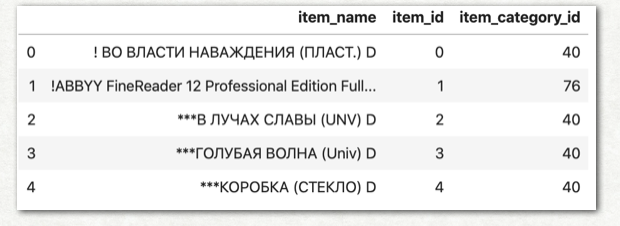
\includegraphics{test.png}
    \caption{Sample figure caption.}
    \label{fig:fig1}
\end{figure}

\subsection{Tables}

See awesome Table~\ref{tab:table}.

\begin{table}
 \caption{Sample table title}
  \centering
  \begin{tabular}{lll}
    \toprule
    \multicolumn{2}{c}{Part}                   \\
    \cmidrule(r){1-2}
    Name     & Description     & Size ($\mu$m) \\
    \midrule
    Dendrite & Input terminal  & $\sim$100     \\
    Axon     & Output terminal & $\sim$10      \\
    Soma     & Cell body       & up to $10^6$  \\
    \bottomrule
  \end{tabular}
  \label{tab:table}
\end{table}

\subsection{Lists}
\begin{itemize}
\item Lorem ipsum dolor sit amet
\item consectetur adipiscing elit. 
\item Aliquam dignissim blandit est, in dictum tortor gravida eget. In ac rutrum magna.
\end{itemize}


%\bibliographystyle{unsrt}  
 
\bibliographystyle{unsrt}  
\bibliography{references}


\end{document}
